% !TEX program = xelatex
% !BIB program = bibtex

\documentclass[aps,pra,preprint,amsmath,amssymb,floatfix]{revtex4-2}

\usepackage{mathtools}
\usepackage{graphicx}
\usepackage{dcolumn}
    \newcolumntype{d}[1]{D{.}{.}{#1}}
\usepackage{url}
\usepackage{bm}
\usepackage{float}
\usepackage[colorlinks,linkcolor=blue,anchorcolor=blue,citecolor=blue,breaklinks=true]{hyperref}
\usepackage{xeCJK}
\usepackage{fontspec}
\setCJKmainfont{標楷體}
\setCJKsansfont{標楷體}
\setCJKmonofont{標楷體}
\raggedbottom
\XeTeXlinebreaklocale "zh"
\XeTeXlinebreakskip = 0pt plus 1pt

\usepackage{xcolor}
\definecolor{codegreen}{rgb}{0,0.6,0}
\definecolor{codegray}{rgb}{0.5,0.5,0.5}
\definecolor{codepurple}{rgb}{0.58,0,0.82}
\definecolor{backcolour}{rgb}{0.95,0.95,0.92}
\usepackage{listings}
\lstset{
    basicstyle=\ttfamily\footnotesize,
    backgroundcolor=\color{backcolour},
    commentstyle=\color{codegreen},
    keywordstyle=\color{magenta},
    numberstyle=\tiny\color{codegray},
    stringstyle=\color{codepurple},
    breaklines=true,
}

\begin{document}

\title{Ising-Model-Based Algorithm for Othello Strategy}
\author{Jiun-Cheng Jiang}
\author{Wen-Ning Wan}
\affiliation{Department of Physics National Tsing Hua University, Taiwan}
\date{\today}

\begin{abstract}
    
\end{abstract}

\maketitle

\section{INTRODUCTION}
\subsection{Othello}
\subsubsection{Rule}
Othello is a two-player strategy board game played on an $8\times8$ board. Each player has pieces, which are black and white. The game starts with four pieces in the middle of the board, two black and two white. The players take turns placing pieces on the board with their assigned color facing up. 

A piece can only be placed on an empty square if it can flip at least one of the opponent's pieces. To flip the opponent's pieces, the new piece must be placed so that an straight (horizontal, vertical, or diagonal) line connects it with at least one of the opponent's pieces. All of the opponent's pieces between the new piece and the connected piece are then flipped to the new piece's color. The object of the game is to have the majority of pieces turned to display your color when the last playable empty square is filled. 

The game ends when neither player has a legal move. The winner is the player with the majority of pieces on the board. If both players have the same number of pieces, the game is a draw.

\subsubsection{Strategy}\label{sec:othello_strategy}
The strategy of Othello is made around the concept of mobility and stability. Mobility is the number of legal moves a player can make. Stability is the number of pieces that cannot be flipped by the opponent.

\paragraph{Grab corner}
Since there is no way to flip the corner pieces, the player who has the corner pieces has a great advantage. Therefore, the corner has the highest stability and has the highest priority to be grabbed.

Additionally, pieces next to the corner piece are also cannot be flipped by the opponent. Therefore, these pieces has the second highest stability.
\par
\paragraph{X square}
The X square is the square surrounding the corner. The player should avoid placing pieces on the X square since it is the most vulnerable square. The opponent can have the chance to occupy the corner if the player places a piece on the X square. Therefore the X square has the lowest stability.
\par
\paragraph{X edge}
The X edge is the edge surrounding the X square. Keeping X edge may make the opponent places pieces on the X square, which help the player to occupy the corner. Therefore, the X edge has high tactical value but low stability.
\par
\paragraph{Danger zone} 
The danger zone is the next rows in from the four edge rows. We should avoid placing pieces on the danger zone since it would help the opponent occupy the edge which has high stability. Therefore, the danger zone has low stability.
\par 
\paragraph{Mobility}
Mobility is the number of moves the player is currently able to make, which has significant weight in the opening of game, but diminishes to zero towards the endgame.
\par

\subsubsection{$\mathbb{Z}2$ Gauge Theory}
Othello can be viewed as discretization of $\mathbb{Z}2$ gauge, since there are some common characteristics. 

Gauge invariant states of $\mathbb{Z}2$ gauge theory is equivalent to the state of Ising model on the board. The flipping on a board corresponds to acting the unit strength magnetic flux on the board. Note that flipping twice makes it back to white due to $\mathbb{Z}2$. \cite{PhysRevD.96.126001}

\subsection{Ising Model}
The Ising model has played an important role in the evolution of ideas in statistical physics and quantum field theory. 

In order to define Ising model, consider a two dimensional square lattice, on each site or node of the lattice we have an atom or a magnet of spin $s_i$. In the Ising model, spins have two possible values, up or down which we map to the numerical values $+1$ or $-1$. The Hamiltonian of the system is given by

\begin{equation}
    \hat{H}=-J\sum_{\langle i,j\rangle}s_is_j-\mu\sum_is_i
\end{equation}

The first term is the spin-spin interaction and for J > 0 the system is ferromagnetic. The minimum energy $E_0$ is obtained for the ground state, which is the unique state in which all spins point in the direction of $\mu$. The minimum energy $E_0$ is obtained for the ground state, which is the unique state in which all spins point in the direction of B. This is equal to
\begin{equation}
    E_0=-(2J+\mu)N
\end{equation}
where N is the number of spins in the system.

The partition function is then given by

\begin{equation}
    Z=\sum_{\{s_i\}}e^{-\beta H_{s_i}}
\end{equation}
where $\{s_i\}\equiv \{s_1,s_2,\dots,s_N\}$ is a spin configuration of the system.

\subsection{Ising-Model-Based Algorithm for Othello Strategy}
\subsubsection{Concepts}
Since the Othello can be viewed as discretization of $\mathbb{Z}2$ gauge, we can use the Ising model to describe the configuration of Othello game. 

\subsubsection{Ansatz of the Hamiltonian of Ising Model for Othello}
We make an ansatz of the Hamiltonian of Ising model for Othello, which is
\begin{equation}
    \hat{H}=-\sum_{i,j}J(i,j)s_is_j-\mu(t)M
\end{equation}
where the first term determined the stability while the second term determined the mobility, and $J(i,j)$ is the interaction between i-piece and j-piece which is
\begin{equation}
    J(i,j) = \sum_p r_ts_p^{(ij)}
\end{equation}
$s_p^{(ij)}$ is the pieces between i-piece and j-piece. $r_t$ is the relevant weight the tactical value of each piece while the middle-16-pieces is set to 1. From Sec.~\ref{sec:othello_strategy}, we can obtain the following relation:
$r_{corner} \geq r_{fixed} \geq r_{X edge} \geq r_{edge}\geq r_{danger zone} \geq r_{X square}$.
The equal sign only happens in endgame and at the time $r_t = 1$. $M$ is the number of moves the
player is currently able to make, and $\mu(t)$ is a time dependent coefficient used to weight the first term and second term, which should be a decay function.

\subsubsection{Evolution Method}
Every time the player makes a move, there would be a state transition. We can view it as that each move imposes a ladder operator on the state and it will lead to the energy change. So we can just calculate the energy change instead of calculating the total energy each time. 

As a result, for each move what we need to consider is the interaction between placing piece and placed pieces and the the change of mobility. And then all we have to do is to find the move which make it to the lowest energy, which is the most stable, in the end.

\subsection{Game Algorithm}
\subsubsection{Minimax Algorithm}
Minimax Algorithm will be the method we use to find the ideal move. To understand Minimax Search, we come across two players. One named Max, and the other named Min. Max eager to get make the with higher score, while Min looks for lower score. This makes them competing one another. We make the score change into a tree diagram, so that we can clearly see how Max and Min would make their choice.\\
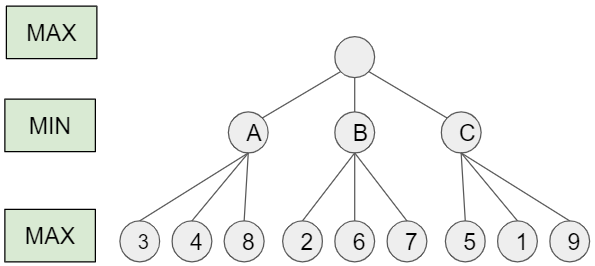
\includegraphics[scale=0.6]{fig/1.png}\\
Every layer indicates the situation one is facing, and the nodes under indicates the move choice they have and the outcome they will get. Take Figure as example, Max has A, B, and C conditions to choose, and each condition then leads to a total of nine choices for Min. As previously mentioned, Min will always pick the minimum result, so we return a value to the node with the minimum value of its successors. Min’s choice is demonstrated under.\\
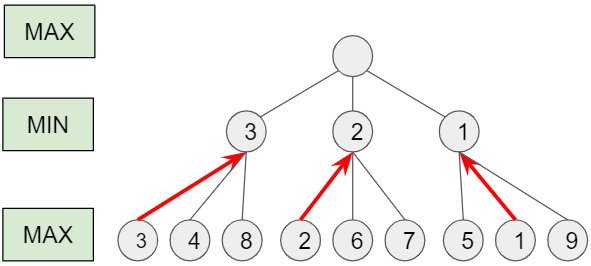
\includegraphics[scale=0.6]{fig/2.png}\\
The main idea of this algorithm is to predict our opponent’s next move. If Max picks the A condition, Min gets 3, 4, 8. Obviously, Min will pick 3 for the minimum result, and same for the other conditions. After the values are passed to the upper layer, Max faces 3, 2, 1, and 3 will be its final choice.\\
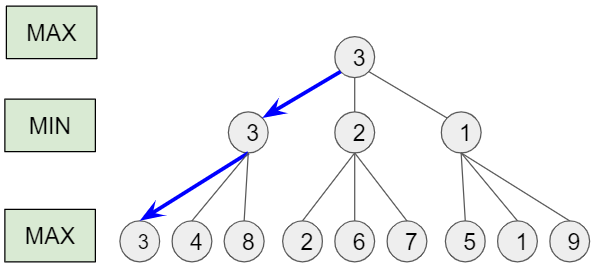
\includegraphics[scale=0.6]{fig/3.png}\\
Now we are clear with the strategy for both side, and the moves are predictable. However, it is predictable only in known layers. If we want to go further depth, it will take up time and memory space. Therefore, we will need the aid of alpha-beta pruning.\\
\subsubsection{Alpha-beta Pruning}
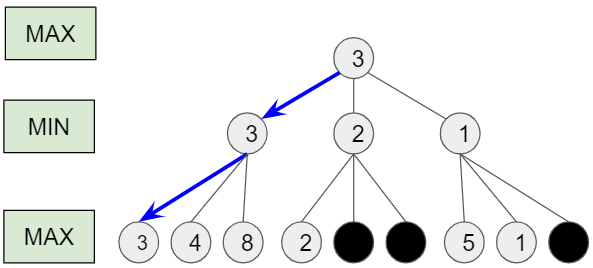
\includegraphics[scale=0.6]{fig/4.png}\\
By pruning, we make the tree diagram smaller. Some nodes in B condition are filled black is because if we look at a layer from left to right, we come across A condition branch, and then the B condition. We meet 2, and since 2 is smaller than 3 from the A condition, we dismiss the rest of the nodes because B condition will no longer be an option for Max. This is how we save time and memory space.
In the former models, we will test with a depth of five, and gradually increase the depth to an acceptable quantity. 

\subsection{Parameters}
After the algorithm had been planned, we have to decide the value of each node. Basically, it will be the Hamilton of the condition. Looking into the formula, we still miss the J and mu. Since the quantity of J and mu will evaluate will the game goes on. For example, mobility is important in the beginning of the game, and less important in the end of the game. We might use a time dependent function, such as exponential, or sigmoid to do the regression of each parameter. This part remains unclear.
\subsection{Dataset}
We will be using the record of 2013 World Othello Championship, which we find it online.\cite{othello_dataset}  It contains 50 fully played game with approximate 60 moves. We will be using them to train and adjust our model.

\section{Code}
\subsection{Othello}



\nocite{*}
\Urlmuskip=0mu plus 2mu\relax
\bibliographystyle{apsrev4-2}
\bibliography{ref}
\end{document}